\documentclass[a4paper,12pt]{article}
\usepackage{standalone}
\usepackage[a4paper, top=0.8in, bottom=0.7in, left=0.8in, right=0.8in]{geometry}
\usepackage{amsmath}
\usepackage{hyperref}
\usepackage{amsfonts}
\usepackage{latexsym}
\usepackage{graphicx}
\usepackage{fancyhdr}
\usepackage{enumitem}
\usepackage{setspace}
\usepackage{tcolorbox}
\usepackage{tikz}
\usepackage{multicol}
\usepackage[defaultfam,tabular,lining]{montserrat} % Font settings for Montserrat

\usepackage{xcolor}  % To use colors
\hypersetup{
    colorlinks=true,   % Activate colored links
    linkcolor=blue,    % Link color for internal links
    urlcolor=blue,     % Link color for URLs
    filecolor=blue,    % Link color for file links
    menucolor=blue,    % Link color for menus
}



\sloppy

\title{}
\date{}
\hyphenpenalty=10000
\exhyphenpenalty=10000

\setlength{\parindent}{0pt}
\pagestyle{fancy}

\setlength{\headheight}{27.11148pt}
\addtolength{\topmargin}{-15.11148pt}

\fancyhf{}
\fancyhead[L]{\textbf{Curriculum D SWB}}
\fancyhead[R]{\includegraphics[width=0.8cm]{Round Logo.png}} % Placeholder for logo
\fancyfoot[C]{\footnotesize © Study Smart Tutors}
\fancyfoot[R]{\thepage}  % Page number in bottom right corner
\fancyfoot[L]{\hyperlink{toc}{Back to Contents}} % Clickable link in bottom left to TOC




\sloppy

% Define a new command for the level letter
\newcommand{\levelLetter}{D}  % Change this letter to update throughout the document

%%%%%%%%%%%%%%%%%%%%%%%%%%%%%%%%%%%%%

\begin{document}

% Title Page
\input{Tutoring Cover Pages/Math Curriculum Materials Cover Pages/Curriculum D Math.tex} % Include the title page content here
\pagenumbering{gobble} 

\hypertarget{toc}{}  % Mark the TOC as a hyperlink target
% Table of Contents
\tableofcontents


\newpage



% Restart page numbering from 1 after TOC
\pagenumbering{arabic}
\pagestyle{fancy}  % Re-enable fancy headers/footers



% Guided Lesson and Problem Set for 3.PAR.3.2, 3.PAR.3.6 (Mapped from 3.OA.A.1, 3.OA.A.3)
\newpage
\section{3.PAR.3.2, 3.PAR.3.6 Guided Lesson}
\input{Grade 3/Grade 3 Guided Lesson/Generic.3.OA.A.1, 3.OA.A.3.GL.tex}

\newpage
\section{3.PAR.3.2, 3.PAR.3.6 Problem Set}
\input{Grade 3/Grade 3 Problem Sets/Generic.3.OA.A.1, 3.OA.A.3.PS.tex}

% Guided Lesson and Problem Set for 3.PAR.3.7 (Mapped from 3.OA.A.4)
\newpage
\section{3.PAR.3.7 Guided Lesson}
\documentclass[11pt]{article} 
\usepackage[a4paper, top=0.8in, bottom=0.7in, left=0.8in, right=0.8in]{geometry}
\usepackage{amsmath}
\usepackage{amsfonts}
\usepackage{latexsym}
\usepackage{graphicx}
\usepackage{fancyhdr}
\usepackage{enumitem}
\usepackage{setspace}
\usepackage{tcolorbox}
\usepackage{textcomp}
\usepackage[defaultfam,tabular,lining]{montserrat} % Font settings for Montserrat

% ChatGPT Directions:
% ----------------------------------------------------------------------
% This template is designed for creating guided lessons that align strictly with specific standards.
% Key points to ensure proper usage:
% 
% 1. **Key Concepts and Vocabulary**:
%    - Include only the concepts necessary for meeting the standards.
%    - Each Key Concept section must align explicitly with the standards being addressed.
%    - If unrelated standards are introduced (e.g., introducing new operations or properties),
%      create additional Key Concept sections labeled "Part 2," "Part 3," etc.
% 2. **Examples**:
%    - Provide concrete worked examples to illustrate the Key Concepts.
%    - These should directly tie back to the Key Concepts presented earlier.
% 3. **Guided Practice**:
%    - Problems should reinforce Key Concepts and Examples.
%    - Allow for ample spacing between problems to give students room for work.
% 4. **Additional Notes**:
%    - Use this section for helpful but non-essential concepts, strategies, or teacher notes.
%    - Examples: Fact families, properties of operations, or alternative explanations.
% 5. **Independent Practice**:
%    - Provide problems for students to practice Key Concepts individually.
% 6. **Exit Ticket**:
%    - Include a reflective or assessment-based question to evaluate student understanding.
% ----------------------------------------------------------------------

\setlength{\parindent}{0pt}
\pagestyle{fancy}

\setlength{\headheight}{27.11148pt}
\addtolength{\topmargin}{-15.11148pt}

\fancyhf{}
%\fancyhead[L]{\textbf{Standard(s): 3.OA.A.4}} % Example standards
\fancyhead[R]{\includegraphics[width=0.8cm]{Round Logo.png}} % Placeholder for logo
\fancyfoot[C]{\footnotesize © Study Smart Tutors}

\sloppy

\title{}
\date{}
\hyphenpenalty=10000
\exhyphenpenalty=10000

\begin{document}

\subsection*{Guided Lesson: Solving for Unknowns in Multiplication and Division}
\onehalfspacing

% Learning Objective Box
\begin{tcolorbox}[colframe=black!40, colback=gray!5, 
coltitle=black, colbacktitle=black!20, fonttitle=\bfseries\Large, 
title=Learning Objective, halign title=center, left=5pt, right=5pt, top=5pt, bottom=15pt]
\textbf{Objective:} Determine the unknown whole number in a multiplication or division equation by understanding the relationship between these operations.
\end{tcolorbox}

\vspace{1em}

% Key Concepts and Vocabulary
\begin{tcolorbox}[colframe=black!60, colback=white, 
coltitle=black, colbacktitle=black!15, fonttitle=\bfseries\Large, 
title=Key Concepts and Vocabulary, halign title=center, left=10pt, right=10pt, top=10pt, bottom=15pt]
\textbf{Key Concepts:}
\begin{itemize}
    \item \textbf{Equations with Unknowns:} In a multiplication or division equation, the unknown can be the product, quotient, or one of the factors (e.g., \(3 \times ? = 12\) or \(? \div 4 = 6\)).
    \item \textbf{Inverse Operations:} Multiplication and division are inverse operations. Knowing one operation helps to solve the other.
    \item \textbf{Fact Families:} A group of related facts can help solve for unknowns. For example, if \(6 \times 4 = 24\), then \(24 \div 6 = 4\) and \(24 \div 4 = 6\).
\end{itemize}
\end{tcolorbox}

\vspace{1em}

% Examples
\begin{tcolorbox}[colframe=black!60, colback=white, 
coltitle=black, colbacktitle=black!15, fonttitle=\bfseries\Large, 
title=Examples, halign title=center, left=10pt, right=10pt, top=10pt, bottom=15pt]
\textbf{Example 1: Solving a Multiplication Equation}
\begin{itemize}
    \item Problem: Solve for \(x\): \(5 \times x = 20\).
    \item Solution: Use division to solve: \(x = 20 \div 5\). \(x = 4\).
\end{itemize}

\textbf{Example 2: Solving a Division Equation}
\begin{itemize}
    \item Problem: Solve for \(y\): \(36 \div y = 9\).
    \item Solution: Use multiplication to solve: \(y \times 9 = 36\). \(y = 36 \div 9 = 4\).
\end{itemize}

\textbf{Example 3: Filling in the Missing Number}
\begin{itemize}
    \item Problem: What number makes this equation true? \(7 \times ? = 49\).
    \item Solution: Divide \(49 \div 7 = 7\). The missing number is \(7\).
\end{itemize}

\textbf{Example 4: Real-Life Scenario}
\begin{itemize}
    \item Problem: A classroom has \(36\) students. They are divided into \(6\) groups. How many students are in each group?
    \item Solution: Divide \(36 \div 6 = 6\). Each group has \(6\) students.
\end{itemize}
\end{tcolorbox}

\vspace{1em}

% Guided Practice
\begin{tcolorbox}[colframe=black!60, colback=white, 
coltitle=black, colbacktitle=black!15, fonttitle=\bfseries\Large, 
title=Guided Practice, halign title=center, left=10pt, right=10pt, top=10pt, bottom=15pt]
\textbf{Solve the following problems with teacher support:}
\begin{enumerate}[itemsep=5em] % Increased spacing for student work
    \item Solve for \(n\): \(8 \times n = 64\).
    \item Write a division equation for: "A total of 45 candies are divided equally into 9 bags. Each bag contains 5 candies."
    \item Solve for the missing number: \(? \div 7 = 3\).
    \item Solve this real-world problem: A gardener plants \(5\) rows of flowers with \(8\) flowers in each row. \(3\) flowers in each row are eaten by bugs. Write an equation and solve for the total flowers left.
\end{enumerate}
\end{tcolorbox}

\vspace{1em}

% Additional Notes
\begin{tcolorbox}[colframe=black!40, colback=gray!5, 
coltitle=black, colbacktitle=black!20, fonttitle=\bfseries\Large, 
title=Additional Notes, halign title=center, left=5pt, right=5pt, top=5pt, bottom=15pt]
\textbf{Note:}
\begin{itemize}
    \item \textbf{Checking Your Work:} Always substitute your solution back into the original equation to verify its correctness.
    \item \textbf{Drawing Models:} Visual models like arrays or number lines can help in understanding multiplication and division equations.
\end{itemize}
\end{tcolorbox}

\vspace{1em}
% Independent Practice Box
\begin{tcolorbox}[colframe=black!60, colback=white, 
coltitle=black, colbacktitle=black!15, fonttitle=\bfseries\Large, 
    title=Independent Practice, halign title=center, left=10pt, right=10pt, top=10pt, bottom=60pt]
\textbf{Solve the following problems independently.}
\begin{enumerate}[itemsep=3em] % Adjust spacing for student work
    \item Solve for \( x \): \( 7 \times x = 42 \).
    
    \item Find the missing number: \( ? \div 8 = 5 \).
    
    \item A baker has 48 cupcakes. She arranges them into boxes, each holding 6 cupcakes. How many boxes does she need?
    
    \item Write a multiplication equation that matches this situation:  
    "A farmer plants 9 rows of carrots with 4 carrots in each row."
    
    \item A student has 36 pencils and gives them equally to 6 friends. How many pencils does each friend get?
    
    \item Solve for \( y \) and check your answer using multiplication: \( y \div 3 = 7 \).
    
    \item Solve for \( z \) and check your answer using division: \( 5z = 35 \).
    
    \item Draw an array to represent \( 5 \times 6 \). How many dots are there?
\end{enumerate}
\end{tcolorbox}


% \vspace{3em}

% Reflection Box
\begin{tcolorbox}[colframe=black!60, colback=white, 
coltitle=black, colbacktitle=black!15, fonttitle=\bfseries\Large, 
title=Exit Ticket, halign title=center, left=10pt, right=10pt, top=10pt, bottom=30pt]
{How can you use multiplication to help solve problems involving division?}

\vspace{3cm}
\end{tcolorbox}

\end{document}


\newpage
\section{3.PAR.3.7 Problem Set}
\documentclass[12pt]{article}
\usepackage[a4paper, top=0.8in, bottom=0.7in, left=0.8in, right=0.8in]{geometry}
\usepackage{amsmath}
\usepackage{amsfonts}
\usepackage{graphicx}
\usepackage{fancyhdr}
\usepackage{tcolorbox}
\usepackage{enumitem}
\usepackage{setspace}
\usepackage[defaultfam,tabular,lining]{montserrat}
\usepackage{xcolor}

\setlength{\parindent}{0pt}
\pagestyle{fancy}

\setlength{\headheight}{27.11148pt}
\addtolength{\topmargin}{-15.11148pt}

\fancyhf{}
%\fancyhead[L]{\textbf{3.OA.A.4: Multiplication and Division Problem Solving}}
\fancyhead[R]{\includegraphics[width=0.8cm]{Round Logo.png}}
\fancyfoot[C]{\footnotesize © Study Smart Tutors}

\sloppy

\title{}
\date{}
\hyphenpenalty=10000
\exhyphenpenalty=10000

\begin{document}

\subsection*{Problem Set: Multiplication and Division Problem Solving}
\onehalfspacing

% Learning Objective Box
\begin{tcolorbox}[colframe=black!40, colback=gray!5, 
coltitle=black, colbacktitle=black!20, fonttitle=\bfseries\Large, 
title=Learning Objective, halign title=center, left=5pt, right=5pt, top=5pt, bottom=15pt]
\textbf{Objective:} Solve multiplication and division problems involving unknown products, group sizes, and numbers of groups using equal groups, arrays, and comparison situations.
\end{tcolorbox}

% Exercises Box
\begin{tcolorbox}[colframe=black!60, colback=white, 
coltitle=black, colbacktitle=black!15, fonttitle=\bfseries\Large, 
title=Exercises, halign title=center, left=10pt, right=10pt, top=10pt, bottom=60pt]
\textbf{Find the missing number in each problem below:}
\begin{enumerate}[itemsep=2em]
    \item \(8 \times \_\_\_ = 56\)  
    \item \(6 \times \_\_\_ = 42\)  
    \item \(45 \div \_\_\_ = 9\)  
    \item \(\_\_\_ \times 4 = 20\)  
    \item \(15 \div \_\_\_ = 5\)  
    \item \(3 \times (\_\_\_ + 5) = 27\)  
    \item \(\_\_\_ \times 5 = 35\)  
    \item \(12 \div \_\_\_ + 6 = 9\)  
    \item \(9 \div \_\_\_ = 3\)  
    \item \(8 \times \_\_\_ = 48\)
\end{enumerate}
\end{tcolorbox}

% Problems Box
\begin{tcolorbox}[colframe=black!60, colback=white, 
coltitle=black, colbacktitle=black!15, fonttitle=\bfseries\Large, 
title=Problems, halign title=center, left=10pt, right=10pt, top=10pt, bottom=60pt]
\begin{enumerate}[start=11, itemsep=5em]
    
    
    \item A gardener plants \(5\) rows of flowers with \(8\) flowers in each row. \(3\) flowers in each row are eaten by bugs. Write an equation to find the total number of flowers left.
    \item A soccer team has \(18\) players. The coach divides them equally into \(3\) teams. Each team gains \(2\) extra players. How many players are now on each team?
    \item A library has \(120\) books. They are placed equally on \(6\) shelves, and \(12\) books are reserved for a display table. Write and solve an equation to find how many books are on each shelf.
    \item A classroom has \(36\) students. The teacher divides them into \(6\) groups. Each group gets \(2\) additional students. How many students are in each group now?

    \item There are \(12\) chairs in a room. If the chairs are arranged equally into \(4\) rows, how many chairs are in each row? Write and solve an equation.
    
    \item If \(27\) apples are arranged in \(9\) rows, how many apples are in each row? Write and solve an equation.
\end{enumerate}
\end{tcolorbox}

\vspace{1em}

% Performance Task Box
\begin{tcolorbox}[colframe=black!60, colback=white, 
coltitle=black, colbacktitle=black!15, fonttitle=\bfseries\Large, 
title=Performance Task: Organizing a Classroom Library, halign title=center, left=10pt, right=10pt, top=10pt, bottom=50pt]
You are organizing books in your classroom library. Here’s what you have:
\begin{itemize}
    \item There are \(48\) books, and you divide them equally among \(6\) shelves.
    \item You add \(5\) extra books to one of the shelves.
    \item There are \(2\) empty bins that can hold up to \(10\) books each.
\end{itemize}
\textbf{Task:}
\begin{enumerate}[itemsep=6em]
    \item How many books are on each shelf before adding extra books?
    \item How many books are on the shelf with the extra books?
    \item Will all the books from the shelf with extras fit into the two bins? Explain why or why not. 
    \vspace{4em}
   
\end{enumerate}
\end{tcolorbox}

\vspace{1em}

% Reflection Box
\begin{tcolorbox}[colframe=black!60, colback=white, 
coltitle=black, colbacktitle=black!15, fonttitle=\bfseries\Large, 
title=Reflection, halign title=center, left=10pt, right=10pt, top=10pt, bottom=100pt]
{How can you use multiplication to help solve problems involving division?}
\end{tcolorbox}


\end{document}


% Guided Lesson and Problem Set for 3.PAR.3.3 (Mapped from 3.OA.B.5, 3.OA.B.6)
\newpage
\section{3.PAR.3.3 Guided Lesson}
\input{Grade 3/Grade 3 Guided Lesson/Generic.3.OA.B.5, 3.OA.B.6.GL.tex}

\newpage
\section{3.PAR.3.3 Problem Set}
\input{Grade 3/Grade 3 Problem Sets/Generic.3.OA.B.5, 3.OA.B.6.PS.tex}

% Guided Lesson and Problem Set for 3.PAR.3.6 (Mapped from 3.OA.C.7)
\newpage
\section{3.PAR.3.6 Guided Lesson}
\input{Grade 3/Grade 3 Guided Lesson/Generic.3.OA.C.7.GL.tex}

\newpage
\section{3.PAR.3.6 Problem Set}
\documentclass[12pt]{article}
\usepackage[a4paper, top=0.8in, bottom=0.7in, left=0.8in, right=0.8in]{geometry}
\usepackage{amsmath}
\usepackage{amsfonts}
\usepackage{latexsym}
\usepackage{graphicx}
\usepackage{fancyhdr}
\usepackage{tcolorbox}
\usepackage{enumitem}
\usepackage{setspace}
\usepackage{multicol}
\usepackage[defaultfam,tabular,lining]{montserrat} % Font settings for Montserrat

% General Comment: Template for creating problem sets in a structured format with headers, titles, and sections.
% This document uses Montserrat font and consistent styles for exercises, problems, and performance tasks.

% -------------------------------------------------------------------
% ChatGPT Directions: 
% 1. Always include a header that dynamically updates based on the standards and topic title.
%    Example: \fancyhead[L]{\textbf{<Standards>: <Topic Title>}}
%
% 2. Subsection titles should always start with "Problem Set:" followed by the topic title.
%    Example: \subsection*{Problem Set: Understanding Multiplication and Division}.
%
% 3. **Section Breakdown**:
%    - **Learning Objective**: A concise statement summarizing the goal of the problem set.
%    - **Exercises**: Focus on procedural fluency with straightforward tasks, organized by question type (e.g., multiplication, division, fill-in-the-blank, mixed operations).
%    - **Problems**: Check for deeper understanding through moderately complex scenarios. Include a variety of question types, such as multi-step problems, tasks requiring reasoning, or comprehensive skill-building beyond word problems.
%    - **Performance Task**: Real-world, open-ended tasks that require multi-step solutions or creative thinking.
%    - **Reflection**: Prompt students to reflect on their strategies and learning.
%
% 4. **Styling with tcolorbox**:
%    - Use the following guidelines for tcolorbox styling:
%        - **Frame color**: black or dark gray (colframe=black!60).
%        - **Background color**: light gray or white (colback=gray!5 or colback=white).
%        - **Title background**: slightly darker gray (colbacktitle=black!15).
%        - **Font style**: Bold and large for titles (fonttitle=\bfseries\Large).
%
% 5. **Content and Alignment**:
%    - Align tasks with the defined standard(s).
%    - Ensure a balance of exercises (procedural), problems (conceptual), and performance tasks (application).
%    - Adjust spacing for student work using \vspace and itemsep as needed.
%
% 6. **Definitions**:
%    - **Exercises**: Develop fluency (e.g., basic computations or simple tasks). Organize into clear groups by question type.
%    - **Problems**: Build understanding with moderately complex applications. Include skill checks, reasoning tasks, or more comprehensive challenges in addition to word problems.
%    - **Performance Tasks**: Require real-world application, design, or explanation.
%
% 7. **Examples**:
%    - For an exercise: "Find the quotient of \(56 \div 8\)."
%    - For a problem: "A student solves \(9 \times 8 = 72\) and claims that \(72 \div 8 = 8\). Is the student correct? Explain why."
%    - For a performance task: "Design a seating arrangement for a classroom using fractions to represent groups."
%
% 8. Use this template for future problem sets and update only the standards, topic title, and content inside each section.
% -------------------------------------------------------------------

\setlength{\parindent}{0pt}
\pagestyle{fancy}

\setlength{\headheight}{27.11148pt}
\addtolength{\topmargin}{-15.11148pt}

\fancyhf{}
%\fancyhead[L]{\textbf{3.OA.C.7: Fluently Multiply and Divide Within 100}} % Header with standards and topic title
\fancyhead[R]{\includegraphics[width=0.8cm]{Round Logo.png}} % Placeholder for logo
\fancyfoot[C]{\footnotesize \textcopyright{} Study Smart Tutors}

\sloppy

\title{}
\date{}
\hyphenpenalty=10000
\exhyphenpenalty=10000

\begin{document}

\subsection*{Problem Set: Fluently Multiply and Divide Within 100}
\onehalfspacing

% Learning Objective Box
\begin{tcolorbox}[colframe=black!40, colback=gray!5, 
coltitle=black, colbacktitle=black!20, fonttitle=\bfseries\Large, 
title=Learning Objective, halign title=center, left=5pt, right=5pt, top=5pt, bottom=15pt]
\textbf{Objective:} Fluently multiply and divide within 100 using strategies based on the properties of operations and the relationship between multiplication and division.
\end{tcolorbox}

% Exercises Box
\begin{tcolorbox}[colframe=black!60, colback=white, 
coltitle=black, colbacktitle=black!15, fonttitle=\bfseries\Large, 
title=Exercises, halign title=center, left=10pt, right=10pt, top=10pt, bottom=30pt]
\textbf{Directions:} Complete the exercises below. Follow the instructions for each group of problems.

% Multiplication and Division
\textbf{Multiply or divide as indicated:}
\begin{multicols}{2}
\begin{enumerate}[itemsep=.25em]
    \item  \(8 \times 7 = \)
    \item  \(6 \times 9 = \)
    \item \(72 \div 8 = \)
    \item  \(36 \div 4 = \)
\end{enumerate}
\end{multicols}

% Fill-in-the-Blank
\textbf{Fill in the blank to make the equation true:}
\begin{enumerate}[resume, itemsep=1em]
    \item \(5 \times \_\_\_ = 35\)
    \item \( \_\_\_ \times 7 = 42\)
    \item \(48 \div \_\_\_ = 6\)
    \item \(\_\_\_ \times 7 = 49\)
\end{enumerate}

% Related Facts
\textbf{Write a related fact:}
\begin{enumerate}[resume, itemsep=2em]
    \item Write a related division fact for \(9 \times 8 = 72\).
    \item Write a related multiplication fact for \(56 \div 7 = 8\).
    \vspace{2em}
\end{enumerate}

% Mixed Operations
\textbf{Solve using the operations provided:}
\begin{enumerate}[resume, itemsep=1em]
    \item \((8 \times 5) - 10\)
    \item \((72 \div 9) + (3 \times 4)\)
\end{enumerate}
\end{tcolorbox}

\vspace{1em}

% Problems Box
\begin{tcolorbox}[colframe=black!60, colback=white, 
coltitle=black, colbacktitle=black!15, fonttitle=\bfseries\Large, 
title=Problems, halign title=center, left=10pt, right=10pt, top=10pt, bottom=60pt]
\textbf{Directions:} Solve the following problems. Show your work where required.

\begin{enumerate}[start=17, itemsep=8em]
    \item A baker bakes 72 cookies and packs them equally into 8 boxes. How many cookies are in each box? Show the division you used to find the answer.
    \item A class has 6 rows of desks, with 9 desks in each row. How many desks are there in total? Show the multiplication you used to find the answer.
    \item A student claims that \(35 \div 5 = 8\). Is the student correct? Explain why or why not.
  
    \item Write and solve a multiplication equation for the problem: "There are 4 packs of markers, each containing 6 markers. How many markers are there in total?"

    \vspace{5em}
\end{enumerate}
\end{tcolorbox}

\vspace{1em}
\newpage
% Performance Task Box
\begin{tcolorbox}[colframe=black!60, colback=white, 
coltitle=black, colbacktitle=black!15, fonttitle=\bfseries\Large, 
title=Performance Task: Organizing an Apple Festival, halign title=center, left=10pt, right=10pt, top=10pt, bottom=50pt]
A community apple festival is preparing gift baskets.

\begin{enumerate}[itemsep=5em]
    \item There are \(90\) apples. If each basket must contain \(10\) apples, how many baskets can be made?
    \item After filling the baskets, \(3\) baskets are donated to a local shelter. How many apples are left?
    \item If the remaining apples are divided equally among \(5\) volunteers, how many apples does each volunteer receive?
 
\end{enumerate}
\vspace{3em}
\end{tcolorbox}

\vspace{1em}

% Reflection Box
\begin{tcolorbox}[colframe=black!60, colback=white, 
coltitle=black, colbacktitle=black!15, fonttitle=\bfseries\Large, 
title=Reflection, halign title=center, left=10pt, right=10pt, top=10pt, bottom=80pt]
How does knowing your multiplication facts help you solve division problems? Share any strategies or patterns you noticed.

\vspace{2cm}
\end{tcolorbox}

\end{document}


% Guided Lesson and Problem Set for 3.PAR.2.2, 3.PAR.3.7 (Mapped from 3.OA.C.8)
\newpage
\section{3.PAR.2.2, 3.PAR.3.7 Guided Lesson}
\input{Grade 3/Grade 3 Guided Lesson/Generic.3.OA.C.8.GL.tex}

\newpage
\section{3.PAR.2.2, 3.PAR.3.7 Problem Set}
\documentclass[12pt]{article}
\usepackage[a4paper, top=0.8in, bottom=0.7in, left=0.8in, right=0.8in]{geometry}
\usepackage{amsmath}
\usepackage{amsfonts}
\usepackage{latexsym}
\usepackage{graphicx}
\usepackage{fancyhdr}
\usepackage{tcolorbox}
\usepackage{enumitem}
\usepackage{setspace}
\usepackage[defaultfam,tabular,lining]{montserrat} % Font settings for Montserrat

% General Comment: Template for creating problem sets in a structured format with headers, titles, and sections.
% This document uses Montserrat font and consistent styles for exercises, problems, and performance tasks.

% -------------------------------------------------------------------
% ChatGPT Directions:
% 1. Always include a header with standards and topic title: \fancyhead[L]{\textbf{<Standards>: <Topic Title>}}.
% 2. Subsection titles should always start with "Problem Set:" followed by the topic title.
% 3. Use tcolorbox for distinct sections: Learning Objective, Exercises, Problems, Performance Task, and Reflection.
% 4. Style guidelines:
%    - Frame color: black or dark gray (colframe=black!60).
%    - Background color: light gray or white (colback=gray!5 or colback=white).
%    - Title background: slightly darker gray (colbacktitle=black!15).
%    - Font style: Bold for titles (fonttitle=\bfseries\Large).
% 5. Ensure a balance of procedural (Exercises), conceptual (Problems), and real-world application tasks (Performance Task).
% -------------------------------------------------------------------

\setlength{\parindent}{0pt}
\pagestyle{fancy}

\setlength{\headheight}{27.11148pt}
\addtolength{\topmargin}{-15.11148pt}

\fancyhf{}
%\fancyhead[L]{\textbf{3.OA.C.8: Solve Two-Step Word Problems Using Four Operations}} % Header with standards and topic title
\fancyhead[R]{\includegraphics[width=0.8cm]{Round Logo.png}} % Placeholder for logo
\fancyfoot[C]{\footnotesize \textcopyright{} Study Smart Tutors}

\sloppy

\title{}
\date{}
\hyphenpenalty=10000
\exhyphenpenalty=10000

\begin{document}

\subsection*{Problem Set: Solve Two-Step Word Problems Using Four Operations}
\onehalfspacing

% Learning Objective Box
\begin{tcolorbox}[colframe=black!40, colback=gray!5, 
coltitle=black, colbacktitle=black!20, fonttitle=\bfseries\Large, 
title=Learning Objective, halign title=center, left=5pt, right=5pt, top=5pt, bottom=15pt]
\textbf{Objective:} Solve two-step word problems using the four operations. Represent these problems using equations with a letter standing for the unknown quantity and assess the reasonableness of answers using estimation.
\end{tcolorbox}

% Exercises Box
\begin{tcolorbox}[colframe=black!60, colback=white, 
coltitle=black, colbacktitle=black!15, fonttitle=\bfseries\Large, 
title=Exercises, halign title=center, left=10pt, right=10pt, top=10pt, bottom=60pt]
\textbf{Directions:} Complete the exercises below. Follow the instructions for each group of problems.

% Basic Computations
\textbf{Solve as indicated:}
\begin{enumerate}[itemsep=2em]
\item \( (5 \times 3) + 10 = \)
    \item \( 45 - 6 \times 4 = \)
    \item \( 25 + (8 \div 2) = \)
    \item \( (7 \times 2) - 5 = \)
    \item \( 36 \div 6 + 12 = \)
    \item \( 10 + (4 \times 3) - 6 = \)
    \item \( 20 \div (2 + 3) = \)
    \item A school has 45 students in the morning class and 35 in the afternoon class. How many students are there in total? 

\end{enumerate}
\end{tcolorbox}


\vspace{1em}

% Problems Box
\begin{tcolorbox}[colframe=black!60, colback=white, 
coltitle=black, colbacktitle=black!15, fonttitle=\bfseries\Large, 
title=Problems, halign title=center, left=10pt, right=10pt, top=10pt, bottom=60pt]
\textbf{Directions:} Solve the following problems. Show your work using pictures, numbers, or words.

\begin{enumerate}[start=6, itemsep=6em]
    \item A baker bakes 24 muffins and sells 10. In the afternoon, they bake 18 more. How many muffins does the baker have now? Show your steps.
    \item A farmer has 60 chickens. They sell 20 chickens and divide the rest equally into 4 pens. How many chickens are in each pen? Show your work.
    \item A gardener plants 5 rows of flowers, with 10 flowers in each row. Later, they remove 4 flowers from each row. How many flowers are left? Use a drawing or numbers to explain your answer.
    \item A basketball team scores 25 points in the first quarter and 35 points in the second quarter. If each basket is worth 5 points, how many baskets did they make? Solve and explain your answer.
    \item A library has 120 books. After giving 8 books to each of 10 classes, how many books remain? Solve and explain.
\end{enumerate}
\vspace{2.5em}
\end{tcolorbox}


\vspace{1em}

% Performance Task Box
\begin{tcolorbox}[colframe=black!60, colback=white, 
coltitle=black, colbacktitle=black!15, fonttitle=\bfseries\Large, 
title=Performance Task: Planning a School Event, halign title=center, left=10pt, right=10pt, top=10pt, bottom=50pt]
You are organizing a school event. Here’s what you know:
\begin{itemize}
    \item 200 students and 20 teachers are attending.
    \item Each person will get 3 slices of pizza.
    \item Pizzas are cut into 8 slices each.
    \item Each pizza costs \$12.
\end{itemize}
\textbf{Task:}
\begin{enumerate}[itemsep=4.5em]
    \item How many total slices of pizza are needed? Show how you found your answer.
    \item How many pizzas do you need to order? Use pictures, numbers, or words to explain your answer.
    \item What is the total cost of the pizzas? Show how you calculated the cost.
    \item The event budget is \$400. How much money will be left, or how much extra will you need? Explain your answer.
\end{enumerate}
\end{tcolorbox}

% Reflection Box
\begin{tcolorbox}[colframe=black!60, colback=white, 
coltitle=black, colbacktitle=black!15, fonttitle=\bfseries\Large, 
title=Reflection, halign title=center, left=10pt, right=10pt, top=10pt, bottom=80pt]
What strategies did you use to solve these two-step word problems? How did equations help you organize the information? What real-world connections did you notice while solving these problems?
\end{tcolorbox}

\end{document}


% Guided Lesson and Problem Set for 3.NR.4.1 (Mapped from 3.NF.A.1)
\newpage
\section{3.NR.4.1 Guided Lesson}
\documentclass[12pt]{article}
\usepackage[a4paper, top=0.8in, bottom=0.7in, left=0.8in, right=0.8in]{geometry}
\usepackage{amsmath}
\usepackage{amsfonts}
\usepackage{latexsym}
\usepackage{graphicx}
\usepackage{fancyhdr}
\usepackage{enumitem}
\usepackage{setspace}
\usepackage{tcolorbox}
\usepackage[defaultfam,tabular,lining]{montserrat} % Font settings for Montserrat

% ChatGPT Directions:
% ----------------------------------------------------------------------
% This template is designed for creating guided lessons that align strictly with specific standards.
% Key points to ensure proper usage:
% 
% 1. **Key Concepts and Vocabulary**:
%    - Include only the concepts necessary for meeting the standards.
%    - Each Key Concept section must align explicitly with the standards being addressed.
%    - If unrelated standards are introduced (e.g., introducing new operations or properties),
%      create additional Key Concept sections labeled ""Part 2,"" ""Part 3,"" etc.
% 2. **Examples**:
%    - Provide concrete worked examples to illustrate the Key Concepts.
%    - These should directly tie back to the Key Concepts presented earlier.
% 3. **Guided Practice**:
%    - Problems should reinforce Key Concepts and Examples.
%    - Allow for ample spacing between problems to give students room for work.
% 4. **Additional Notes**:
%    - Use this section for helpful but non-essential concepts, strategies, or teacher notes.
%    - Examples: Fact families, properties of operations, or alternative explanations.
% 5. **Independent Practice**:
%    - Provide problems for students to practice Key Concepts individually.
% 6. **Exit Ticket**:
%    - Include a reflective or assessment-based question to evaluate student understanding.
% ----------------------------------------------------------------------

\setlength{\parindent}{0pt}
\pagestyle{fancy}

\setlength{\headheight}{27.11148pt}
\addtolength{\topmargin}{-15.11148pt}

\fancyhf{}
%\fancyhead[L]{\textbf{Standard(s): 3.NF.A.1}}
\fancyhead[R]{\includegraphics[width=0.8cm]{Round Logo.png}} % Placeholder for logo
\fancyfoot[C]{\footnotesize © Study Smart Tutors}

\sloppy

\title{}
\date{}
\hyphenpenalty=10000
\exhyphenpenalty=10000

\begin{document}

\subsection*{Guided Lesson: Understanding Fractions as Parts of a Whole}
\onehalfspacing

% Learning Objective Box
\begin{tcolorbox}[colframe=black!40, colback=gray!5, 
coltitle=black, colbacktitle=black!20, fonttitle=\bfseries\Large, 
title=Learning Objective, halign title=center, left=5pt, right=5pt, top=5pt, bottom=15pt]
\textbf{Objective:} Understand fractions as parts of a whole and represent them on a number line.
\end{tcolorbox}

\vspace{1em}

% Key Concepts and Vocabulary
\begin{tcolorbox}[colframe=black!60, colback=white, 
coltitle=black, colbacktitle=black!15, fonttitle=\bfseries\Large, 
title=Key Concepts and Vocabulary, halign title=center, left=10pt, right=10pt, top=10pt, bottom=15pt]
\textbf{Key Concepts:}
\begin{itemize}
    \item \textbf{Fraction as Part of a Whole:} A fraction represents one or more equal parts of a whole. For example, \( \frac{1}{4} \) represents one part out of four equal parts.
    \item \textbf{Number Line Representation:} Fractions can be shown on a number line by dividing the segment between 0 and 1 into equal parts.
    \item \textbf{Numerator and Denominator:}
    \begin{itemize}
        \item \textbf{Numerator:} The top number shows how many parts are taken.
        \item \textbf{Denominator:} The bottom number shows the total number of equal parts.
    \end{itemize}
    \item \textbf{Simplest Form:} A fraction is in its simplest form when the numerator and denominator share no common factors other than 1.
    \item \textbf{Equivalence:} Fractions like \( \frac{2}{4} \) and \( \frac{1}{2} \) represent the same part of a whole.
\end{itemize}
\end{tcolorbox}

\vspace{1em}

% Examples
\begin{tcolorbox}[colframe=black!60, colback=white, 
coltitle=black, colbacktitle=black!15, fonttitle=\bfseries\Large, 
title=Examples, halign title=center, left=10pt, right=10pt, top=10pt, bottom=15pt]
\textbf{Example 1: Fraction as a Part of a Whole}
\begin{itemize}
    \item Problem: A pizza is divided into 8 equal slices. If you eat 3 slices, what fraction of the pizza have you eaten?
    \item Solution: You have eaten \( \frac{3}{8} \) of the pizza.
\end{itemize}

\textbf{Example 2: Representing Fractions on a Number Line}
\begin{itemize}
    \item Problem: Divide the segment from 0 to 1 into 4 equal parts and mark \( \frac{3}{4} \) on the number line.
    \item Solution: Draw a number line from 0 to 1. Divide it into 4 equal parts. Count 3 parts starting from 0 and mark \( \frac{3}{4} \).
\end{itemize}

\textbf{Example 3: Simplifying Fractions}
\begin{itemize}
    \item Problem: Simplify \( \frac{6}{8} \).
    \item Solution: Divide the numerator and denominator by their greatest common factor (2). \( \frac{6}{8} = \frac{3}{4} \).
\end{itemize}

\textbf{Example 4: Equivalence of Fractions}
\begin{itemize}
    \item Problem: Show that \( \frac{2}{5} \) and \( \frac{4}{10} \) are equivalent.
    \item Solution: Multiply the numerator and denominator of \( \frac{2}{5} \) by 2: \( \frac{2}{5} = \frac{4}{10} \).
\end{itemize}
\end{tcolorbox}

\vspace{1em}

% Guided Practice
\begin{tcolorbox}[colframe=black!60, colback=white, 
coltitle=black, colbacktitle=black!15, fonttitle=\bfseries\Large, 
title=Guided Practice, halign title=center, left=10pt, right=10pt, top=10pt, bottom=150pt]
\textbf{Solve the following problems with teacher support:}
\begin{enumerate}[itemsep=5em] % Increased spacing for student work
    \item A cake is divided into 6 equal parts. If you eat 2 parts, what fraction of the cake have you eaten? Represent this fraction on a number line.
    \item Divide the segment from 0 to 1 into 5 equal parts. Mark \( \frac{2}{5} \) and \( \frac{4}{5} \) on the number line.
    \item A ribbon is cut into 10 equal pieces. If you use 7 pieces, what fraction of the ribbon have you used? Represent it on a number line.
    \item Simplify the fraction \( \frac{4}{8} \). Explain your reasoning.
    \item Show that \( \frac{3}{6} \) is equivalent to \( \frac{1}{2} \). Use a number line or visual representation to explain.
\end{enumerate}
\end{tcolorbox}

\vspace{1em}

% Additional Notes
\begin{tcolorbox}[colframe=black!40, colback=gray!5, 
coltitle=black, colbacktitle=black!20, fonttitle=\bfseries\Large, 
title=Additional Notes, halign title=center, left=5pt, right=5pt, top=5pt, bottom=15pt]
\textbf{Note:}
\begin{itemize}
    \item \textbf{Unit Fractions:} A fraction where the numerator is 1 (e.g., \( \frac{1}{2}, \frac{1}{3} \)). These are the building blocks of other fractions.
    \item \textbf{Multiple Representations:} Use drawings, number lines, or other visual aids to deepen understanding.
\end{itemize}
\end{tcolorbox}

\vspace{1em}

% Independent Practice
\begin{tcolorbox}[colframe=black!60, colback=white, 
coltitle=black, colbacktitle=black!15, fonttitle=\bfseries\Large, 
title=Independent Practice, halign title=center, left=10pt, right=10pt, top=10pt, bottom=100pt]
\textbf{Solve the following problems independently:}
\begin{enumerate}[itemsep=5em] % Increased spacing for student work
    \item A chocolate bar is divided into 12 equal parts. If you eat 5 parts, what fraction of the chocolate bar have you eaten?
    \item Mark \( \frac{1}{3}, \frac{2}{3} \), and \( 1 \) on a number line divided into 3 equal parts.
    \item A rope is cut into 8 equal sections. If you use 6 sections, what fraction of the rope have you used? Show this fraction on a number line.
    \item Simplify \( \frac{9}{12} \) and explain your steps.
    \item Create your own problem involving fractions and solve it.
\end{enumerate}
\end{tcolorbox}

\vspace{3 cm}
% Exit Ticket
\begin{tcolorbox}[colframe=black!60, colback=white, 
coltitle=black, colbacktitle=black!15, fonttitle=\bfseries\Large, 
title=Exit Ticket, halign title=center, left=10pt, right=10pt, top=10pt, bottom=15pt]
\textbf{Answer the following question:}
\begin{itemize}
    \item How can fractions be represented on a number line? Provide an example.
    \item Why is it important to simplify fractions? Share one real-world example.
\end{itemize}
\vspace{5cm}
\end{tcolorbox}

\end{document}


\newpage
\section{3.NR.4.1 Problem Set}
\documentclass[12pt]{article}
\usepackage[a4paper, top=0.8in, bottom=0.7in, left=0.8in, right=0.8in]{geometry}
\usepackage{amsmath}
\usepackage{amsfonts}
\usepackage{latexsym}
\usepackage{graphicx}
\usepackage{fancyhdr}
\usepackage{tcolorbox}
\usepackage{enumitem}
\usepackage{setspace}
\usepackage[defaultfam,tabular,lining]{montserrat} % Font settings for Montserrat
\usepackage{tikz} % For number line and visual tasks

% General Comment: Template for creating problem sets aligned with a specific standard.

\setlength{\parindent}{0pt}
\pagestyle{fancy}

\setlength{\headheight}{27.11148pt}
\addtolength{\topmargin}{-15.11148pt}

\fancyhf{}
%\fancyhead[L]{\textbf{3.NF.A.1: Understanding Fractions as Numbers}} % Header with standards and topic title
\fancyhead[R]{\includegraphics[width=0.8cm]{Round Logo.png}} % Placeholder for logo
\fancyfoot[C]{\footnotesize © Study Smart Tutors}

\sloppy

%\newcommand{\dfrac}[2]{\displaystyle\frac{#1}{#2}}

\title{}
\date{}
\hyphenpenalty=10000
\exhyphenpenalty=10000

\begin{document}

\subsection*{Problem Set: Understanding Fractions as Numbers}
\onehalfspacing

% Learning Objective Box
\begin{tcolorbox}[colframe=black!40, colback=gray!5, 
coltitle=black, colbacktitle=black!20, fonttitle=\bfseries\Large, 
title=Learning Objective, halign title=center, left=5pt, right=5pt, top=5pt, bottom=15pt]
\textbf{Objective:} Understand fractions as numbers by interpreting and representing fractions on number lines and visual models.

\end{tcolorbox}
% Exercises Box
\begin{tcolorbox}[colframe=black!60, colback=white, 
coltitle=black, colbacktitle=black!15, fonttitle=\bfseries\Large, 
title=Exercises, halign title=center, left=10pt, right=10pt, top=10pt, bottom=5pt]
\begin{enumerate}[itemsep=1.5em]
    \item Write the fraction that represents \(3\) shaded parts out of \(4\) total parts. 
    \item Mark the fraction \(\displaystyle\frac{1}{2}\) on the number line below.  

    \begin{center}
        \begin{tikzpicture}[x=2cm, y=1cm]
            % Number line
            \draw[thick, ->] (0,0) -- (2,0);
            % Major ticks
            \foreach \x in {0,1,2} {
                \draw[thick] (\x,0.1) -- (\x,-0.1) node[below] {\x};
            }
            % Minor ticks
            \foreach \x in {0.5,1.5} {
                \draw[thick] (\x,0.05) -- (\x,-0.05);
            }
        \end{tikzpicture}
    \end{center}

    \item Write \(\displaystyle\frac{3}{6}\) in simplest form.
    \item Divide the shape below into \(4\) equal parts. \\Shade \(3\) of them to represent \(\displaystyle \frac{3}{4}\).  

    \begin{center}
        \begin{tikzpicture}
            \draw[thick] (0,0) rectangle (4,2); % Draw rectangle
        \end{tikzpicture}
    \end{center}

    \item Write the fraction represented by the point marked on the number line below.

    \begin{center}
        \begin{tikzpicture}[x=2cm, y=1cm]
            % Number line
            \draw[thick, ->] (0,0) -- (2,0);
            % Major ticks
            \foreach \x in {0,1,2} {
                \draw[thick] (\x,0.1) -- (\x,-0.1) node[below] {\x};
            }
            % Minor ticks
            \foreach \x in {.25, 0.5, .75, 1.25, 1.5, 1.75} {
                \draw[thick] (\x,0.05) -- (\x,-0.05);
            }
            % Mark fraction
            \filldraw[red] (1.5,0) circle (3.5pt)  ;
        \end{tikzpicture}
    \end{center}

    \item What fraction is equivalent to \(\displaystyle\frac{2}{4}\)? Write two examples.
    \item Convert \(\displaystyle \frac{5}{10} \) to a decimal.
    \item Write the fraction that represents \(7\) shaded parts out of \(10\) total parts.
\end{enumerate}
 \vspace{2em}
\end{tcolorbox}

\vspace{1cm}

% Problems Box
\begin{tcolorbox}[colframe=black!60, colback=white, 
coltitle=black, colbacktitle=black!15, fonttitle=\bfseries\Large, 
title=Problems, halign title=center, left=10pt, right=10pt, top=10pt, bottom=60pt]
\begin{enumerate}[start=9, itemsep=6em]
    \item Place the following fractions on the number line: \(\displaystyle\frac{1}{3}, \frac{2}{3}, \frac{1}{6}, \frac{5}{6}\).

   \begin{center}
    \begin{tikzpicture}[x=7cm, y=2.5cm] % Adjust x and y scaling here
        % Number line
        \draw[thick, -] (0,0) -- (1,0);
        % Major ticks
        \foreach \x in {0,1} {
            \draw[thick] (\x,0.1) -- (\x,-0.1) node[below] {\x};
        }
        % Minor ticks
        \foreach \x in {0.166,0.333,0.5,0.666,0.833} {
            \draw[thick] (\x,0.05) -- (\x,-0.05);
        }
    \end{tikzpicture}
\end{center}


    \item A pie is cut into \(8\) equal slices. You eat \(3\) slices. Write the fraction of the pie you ate. Is this fraction greater than or less than \(\displaystyle\frac{1}{2}\)? Explain.
    \item Compare the fractions \(\displaystyle\frac{4}{8}\) and \(\dfrac{3}{4}\). Use \(>\), \(<\), or \(=\) to fill in the blank. Explain your reasoning. \vspace{0.5cm}\\ \(\dfrac{4}{8} \quad \_\_\_\quad \frac{3}{4}\).
    
    \item Show \(\dfrac{2}{5}\) and \(\dfrac{4}{10}\) on a number line. Are they equivalent fractions? Explain why.
    \item Convert the fraction \(\dfrac{11}{4}\) into a mixed number. Then plot it on the number line below.

    \begin{center}
        \begin{tikzpicture}[x=1.5cm, y=1cm]
            % Number line
            \draw[thick, ->] (0,0) -- (5,0);
            % Major ticks
            \foreach \x in {0,1,2,3,4,5} {
                \draw[thick] (\x,0.1) -- (\x,-0.1) node[below] {\x};
            }
        \end{tikzpicture}
    \end{center}
\end{enumerate}
\end{tcolorbox}

\vspace{1em}

% Performance Task Box
\begin{tcolorbox}[colframe=black!60, colback=white, 
coltitle=black, colbacktitle=black!15, fonttitle=\bfseries\Large, 
title=Performance Task: Sharing a Cake, halign title=center, left=10pt, right=10pt, top=10pt, bottom=50pt]
You are sharing a cake equally among \(5\) friends. The cake is cut into \(10\) slices.
\begin{enumerate}[itemsep=7em]
    \item Write a fraction that represents how much cake each friend gets.
    \item If you eat \(2\) of your slices, what fraction of the cake do you have left?
    \item Explain how you could use a number line to represent this situation.
    \vspace{3cm}
\end{enumerate}
\end{tcolorbox}

\vspace{1em}

% Reflection Box
\begin{tcolorbox}[colframe=black!60, colback=white, 
coltitle=black, colbacktitle=black!15, fonttitle=\bfseries\Large, 
title=Reflection, halign title=center, left=10pt, right=10pt, top=10pt, bottom=80pt]
How does understanding fractions as numbers help you solve real-world problems? Share one example where fractions can be useful in everyday life.

\vspace{3cm}

\end{tcolorbox}

\end{document}


\end{document}


